%basics of the document
\documentclass[12pt]{article}%font size and document style
\renewcommand{\baselinestretch}{1.5}%1.5 line spaceing
\usepackage{geometry}%marginals
\geometry{a4paper,
 left=35mm,
right=25mm,
 top=25mm,
bottom=25mm}

\usepackage[skip=12pt]{parskip} % no intend, but a little space between paragraphs

\usepackage{graphicx}%package for adding photos

\usepackage{subcaption}%custom caption
\DeclareCaptionFormat{custom}
{%
    \linespread{1.0}\selectfont\footnotesize{#1#2 #3}
}
\DeclareCaptionLabelSeparator{custom}{.}
\captionsetup{format=custom, labelsep=custom}

\setlength{\textfloatsep}{30pt plus 2.0pt minus 4.0pt}
\setlength{\intextsep}{30pt plus 2.0pt minus 4.0pt}

\usepackage{eurosym}%euro

\usepackage{wrapfig}%kuvien wrappaus

\usepackage{amsmath}%equation settings package

\usepackage{array}%package for editing table widths

\usepackage{xcolor}%different colors for text

\usepackage[linkbordercolor=white]{hyperref}%package for creating hyperinks

\usepackage{lipsum}%package for creating text

\usepackage{lastpage} %package for getting number of last page

\usepackage[ddmmyyyy]{datetime} 
\renewcommand{\dateseparator}{.} %style of \today command

%biblatex bibtex reference package. Note that backend is biber not bibtex.
\usepackage[style=authoryear, maxbibnames=99, giveninits=true, dashed=False, backend=biber, minnames=1, maxcitenames=2, uniquelist=false, uniquename=false]{biblatex}
\addbibresource{references.bib}%single bib file of all the references

%reference list settings
\DeclareNameAlias{sortname}{family-given}
\usepackage{xpatch,filecontents}
\xpatchbibmacro{date+extradate}{%no brackets around year
  \printtext[parens]%
}{%
  \setunit*{\space}%only space between name and last author
  \printtext%
}{}{} 

% no oxford comma
\AtBeginBibliography{%
  \renewcommand*{\finalnamedelim}{\addspace and\space}%
  \renewcommand*{\finalandcomma}{}%
}

\makeatletter%no cursive

\renewrobustcmd*{\mkbibemph}{}
\protected\long\def\blx@imc@mkbibemph#1{#1}
\makeatother

\DeclareFieldFormat{pages}{#1}%no pp before pages


%no quetation marks on title of the reference
\DeclareFieldFormat[article]{title}{#1}
\DeclareFieldFormat[inproceedings]{title}{#1}
\DeclareFieldFormat[inbook]{title}{#1}
\DeclareFieldFormat[thesis]{title}{#1}

\renewbibmacro{in:}{}%no in
\AtEveryBibitem{\clearfield{number}}%no volume number
\DeclareNameFormat{customauthor}{%custom author
  \namepartfamily
  \usebibmacro{name:andothers}}

%pagenumber position
\usepackage{fancyhdr} % Custom headers and footers
\pagestyle{fancyplain} % Makes all pages in the document conform to the custom headers and footers
\fancyhead[L]{}% Empty left header
\fancyhead[C]{} % Page numbering for center header  
\fancyhead[R]{}% Empty right header
\fancyfoot[L]{}% Empty left footer
\fancyfoot[C]{}% Empty center footer
\fancyfoot[R]{}% Empty left footer
\renewcommand{\headrulewidth}{0pt}%no line
\setlength{\headheight}{14.5pt}

%section subsection and others style.
\usepackage{titlesec}
\usepackage{titletoc}
\titleformat{\section}
  {\bfseries\MakeUppercase}
  {\thesection}{1em}{}
\titleformat{\subsection}
  {\bfseries}
  {\thesubsection}{1em}{}
\titleformat{\subsubsection}
  {\itshape}
  {\thesubsubsection}{1em}{}

\renewcommand{\thesection}{\arabic{section}.}
\renewcommand{\thesubsection}{\thesection\arabic{subsection}.}
\renewcommand{\thesubsubsection}{\thesubsection\arabic{subsubsection}.}

\titlespacing*{\section}{0pt}{30pt plus 5pt minus 5pt}{5 pt plus 1pt minus 1pt}

\usepackage{tocloft}
\setlength{\cftbeforesubsecskip}{0pt}
\setlength{\cftbeforesecskip}{5pt}

%\usepackage{setspace}

%add your own commands here
\newcommand{\aste}{^{\circ}}%command  for degree mark
\newcommand{\om}{\Omega\text{m}}

\usepackage[table]{xcolor} %table co



\begin{document}
\frenchspacing
%%%%%%%%%%%%%%%%%%%%%%%%%%%%%%%%%%%%%%%%%%%%%%%%%%%%%%%%%%%%%%%%%%%%%%%%%%%%%%%%%%%%%%%%%%%%%%%%%%%%%%%%%%%%%%%%%%%%%%%%%%%%%%%%%%%%%%%%%%%%%%%%%%%%%%%%%%%%%%%%%%%%%%%%%%%%%%%%%%
\begin{titlepage}
\begin{center}
\begin{figure}[h]
\centering
\vspace{1cm}

\includegraphics[width=0.25\linewidth]{hy.jpg}
\end{figure}
\vspace*{3cm}
\textbf{Master's thesis}\\
\bigskip

\textbf{Master's programme in Geology and Geophysics}\\
\vspace*{1cm}

Title, title, title and title using title method in title region

Author (You)

\the\year
\vspace*{2cm}

Supervisors:\\
Professor Great Authority\\
Associate Professor Science Maker\\
\vspace*{2cm}

Master’s Programme in Geology and Geophysics 

Faculty of Science
\end{center}
\end{titlepage}

%%%%%%%%%%%%%%%%%%%%%%%%%%%%%%%%%%%%%%%%%%%%%%%%%%%%%%%%%%%%%%%%%%%%%%

\begin{figure}[h]
\vspace{-2cm}
\hspace{-3cm}

\includegraphics[width=0.4\linewidth]{matlu_logo}
\end{figure}

\begin{tabular}{| c | c  | c | c | c | c |}
\hline
\multicolumn{3}{| p{0.45\linewidth} }{\textbf{Faculty:} Faculty of science} & \multicolumn{3}{| p{0.45\linewidth} |}{\textbf{Degree programme:} Master's programme in Geology and Geophysics}\\
\hline
\multicolumn{6}{| p{0.9\linewidth} |}{\textbf{Study track:} }\\
\hline
\multicolumn{6}{| p{0.9\linewidth} |}{\textbf{Author:} }\\
\hline
\multicolumn{6}{| p{\linewidth} |}{\textbf{Title:} }\\
\hline
\multicolumn{2}{| p{0.3\linewidth} }{\textbf{Level:} Master's thesis} & \multicolumn{2}{| p{0.3\linewidth} |}{\textbf{Month and year:} \the\month/\the\year} & \multicolumn{2}{| p{0.3\linewidth} |}{\textbf{Number of pages:} \pageref{LastPage}}\\
\hline
\multicolumn{6}{| p{0.9\linewidth} |}{\textbf{Abstract:} \lipsum[1-1] }\\
\hline
\multicolumn{6}{| p{0.9\linewidth} |}{\textbf{Keywords:} }\\
\hline
\multicolumn{6}{| p{0.9\linewidth} |}{\textbf{Where deposited:} e-thesis}\\
\hline
\multicolumn{6}{| p{0.9\linewidth} |}{\textbf{Additional information:}}\\
\hline
\end{tabular}
\newpage

\begin{figure}[h]
\vspace{-2cm}
\hspace{-3cm}

\includegraphics[width=0.4\linewidth]{matlu_logo}
\end{figure}

\begin{tabular}{| c | c  | c | c | c | c |}
\hline
\multicolumn{3}{| p{0.45\linewidth} }{\textbf{Tiedekunta:} Matemaattis-luonnontieteellinen tiedekunta} & \multicolumn{3}{| p{0.45\linewidth} |}{\textbf{Koulutusohjelma:} Geologian ja Geo\-fysiikan maisteriohjelma}\\
\hline
\multicolumn{6}{| p{0.9\linewidth} |}{\textbf{Opintosuunta:} }\\
\hline
\multicolumn{6}{| p{0.9\linewidth} |}{\textbf{Tekijä:} }\\
\hline
\multicolumn{6}{| p{0.9\linewidth} |}{\textbf{Työn nimi:}} \\
\hline
\multicolumn{2}{| p{0.3\linewidth} }{\textbf{Työn taso:} Maisteritutkielma} & \multicolumn{2}{| p{0.3\linewidth} |}{\textbf{Kuukausi ja vuosi:} \the\month/\the\year} & \multicolumn{2}{| p{0.3\linewidth} |}{\textbf{Sivumäärä:} \pageref{LastPage}}\\
\hline
\multicolumn{6}{| p{1\linewidth} |}{\textbf{Tiivistelmä:} \lipsum[1-1] }\\
\hline
\multicolumn{6}{| p{0.9\linewidth} |}{\textbf{Avainsanat:} }\\
\hline
\multicolumn{6}{| p{0.9\linewidth} |}{\textbf{Säilytyspaikka:} e-thesis}\\
\hline
\multicolumn{6}{| p{0.9\linewidth} |}{\textbf{Muita tietoja:}}\\
\hline
\end{tabular}
\newpage


%%%%%%%%%%%%%%%%%%%%%%%%%%%%%%%%%%%%%%%%%%%%%%%%%%%%%%%%%%%%%%%%%%%%%%
\tableofcontents
\newpage


%%%%%%%%%%%%%%%%%%%%%%%%%%%%%%%%%%%%%%%%%%%%%%%%%%%%%%%%%%%%%%%%%%%%%%

%start of the page numbering
\fancyhead[C]{\thepage}
\setcounter{page}{4}

\section{TUTORIAL}
I use program called TeXworks. It is available at least for Windws and Linux. Any \LaTeX{} editor should work, so use whatever you want.

Link to the github page of this file \href{https://github.com/Alekzanteri/hy_geo_latex}{github.com/Alekzanteri/hy\_geo\_latex}.

\subsection{References}
There is two custom cite commands that should follow graduopas. \textbackslash citei cretes citation such as \citei{example1} \textbackslash citeii creates citation \citeii{example2} 

\subsection{Figure example}
See Figure \ref{example}. 
\begin{figure}[h]
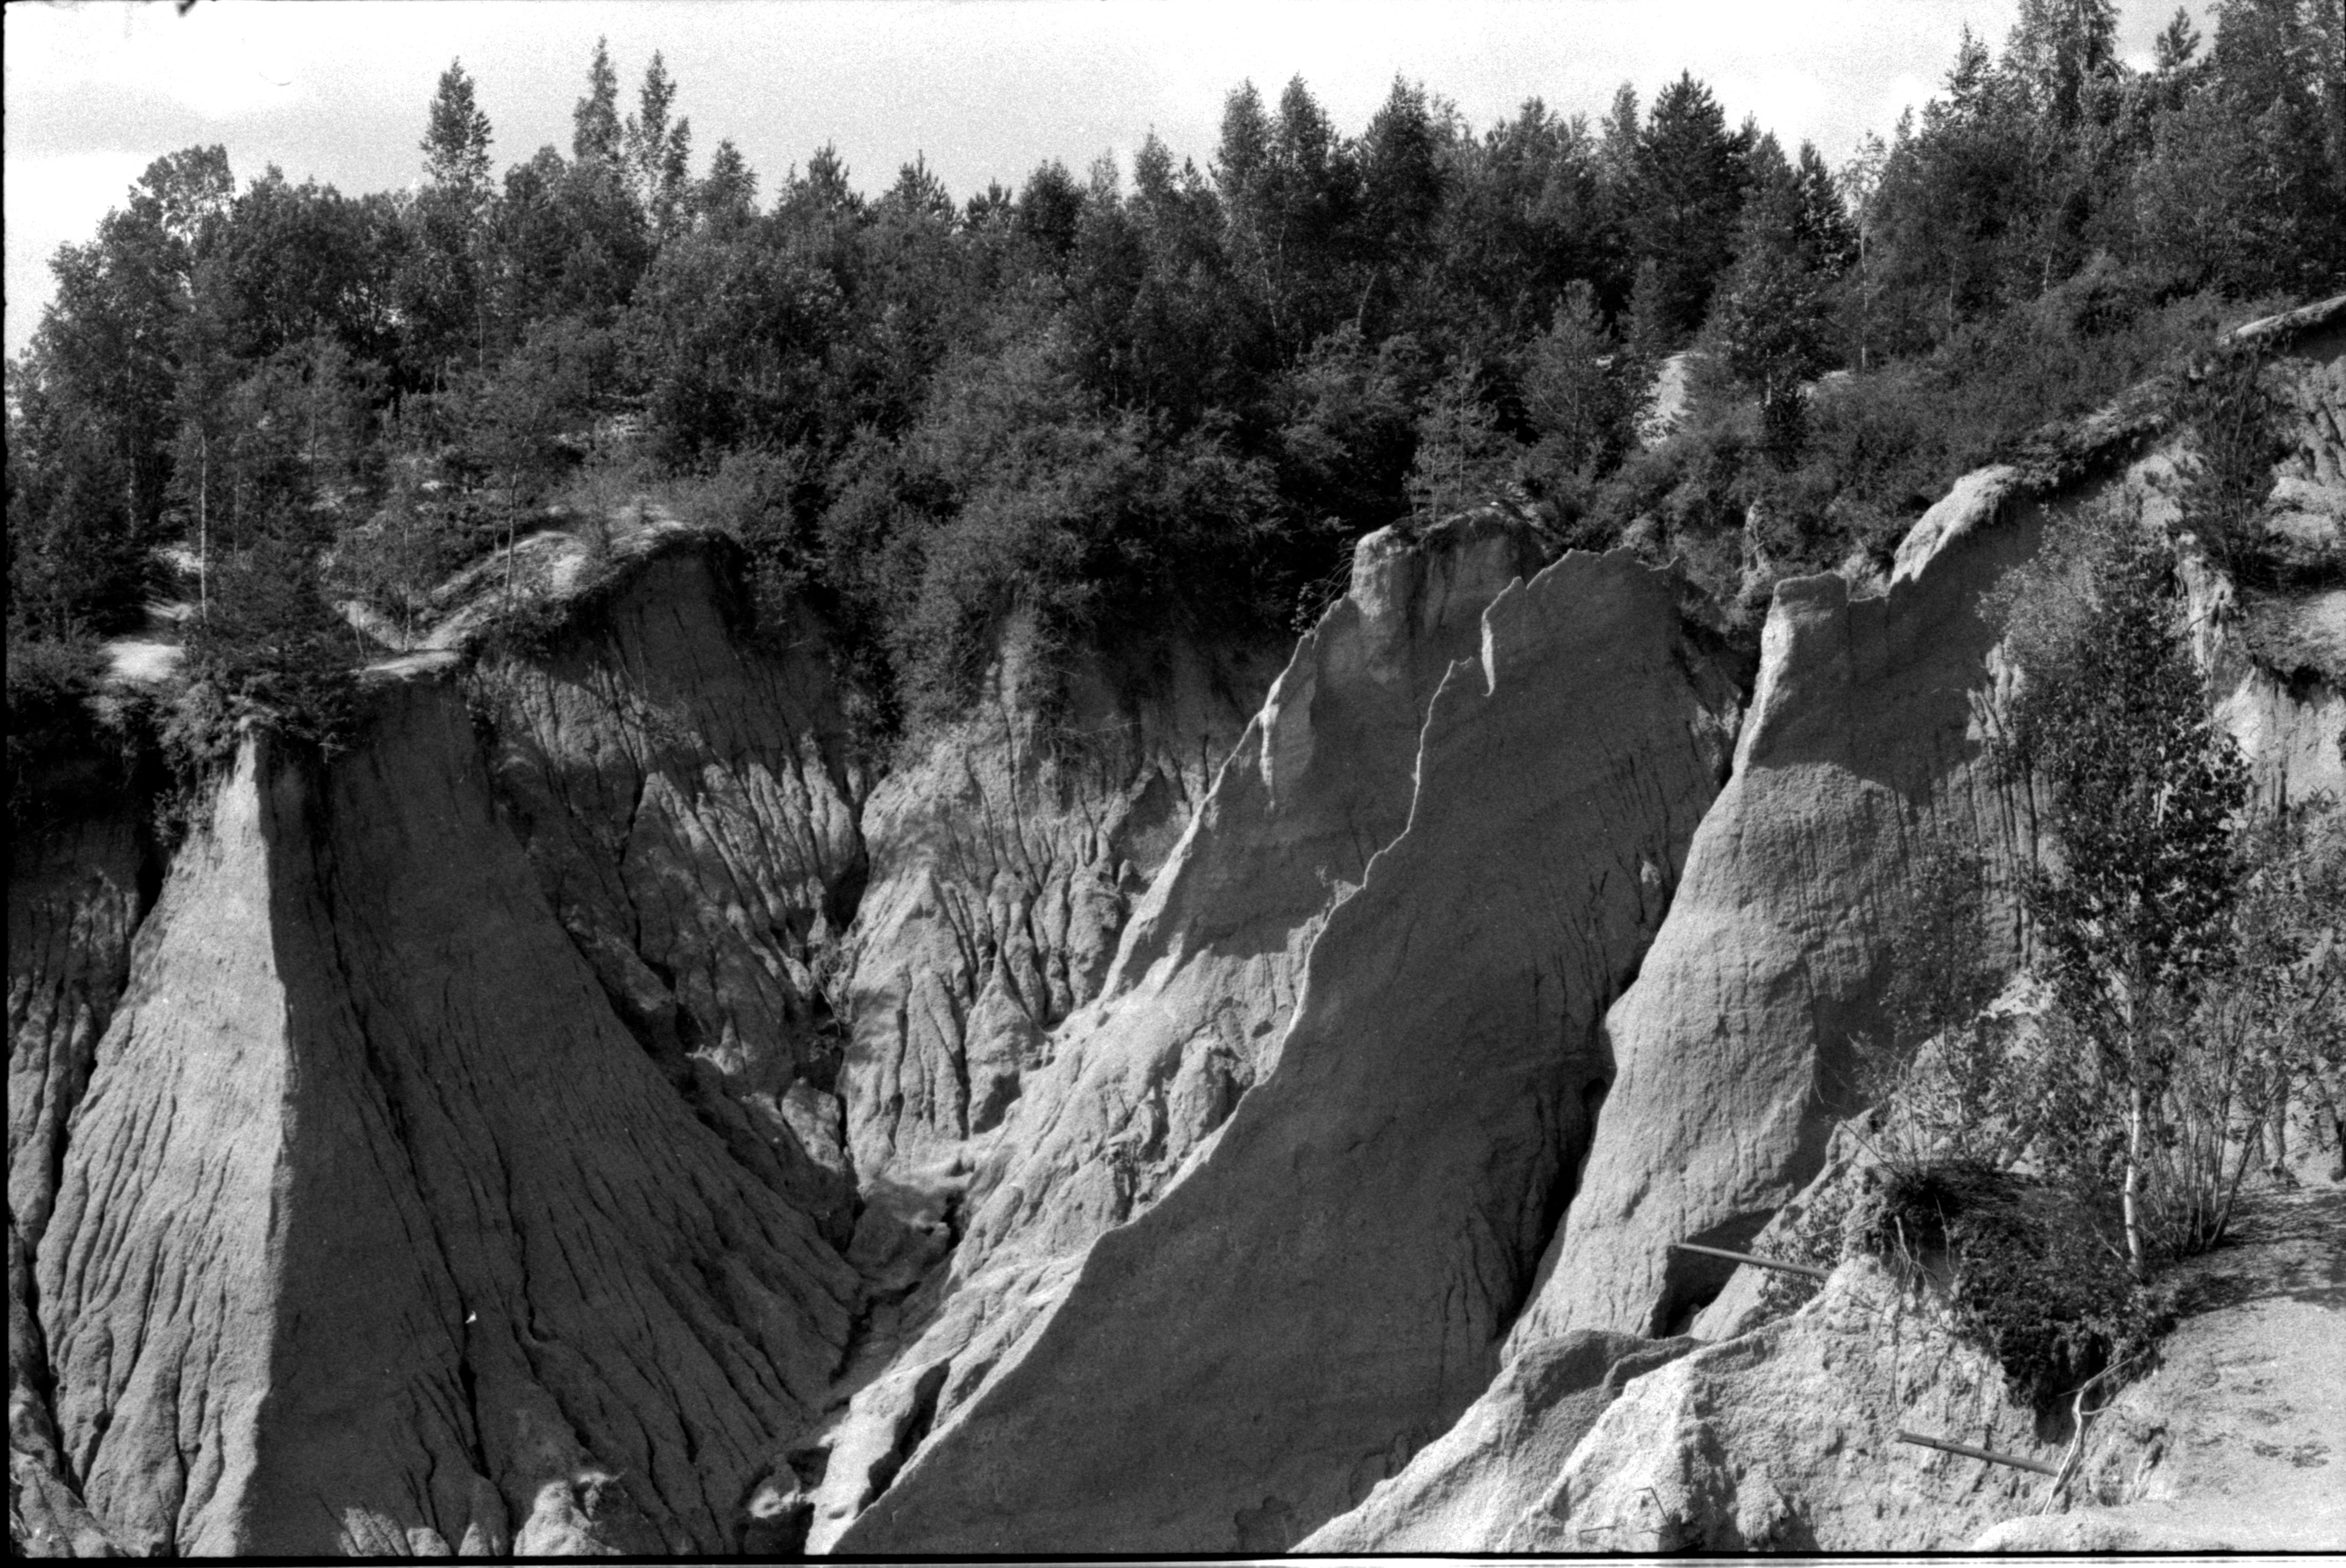
\includegraphics[alt={Olympus OM-10, Fomapan 200}, width=\linewidth]{example.jpg}
\caption{Erosional structures in Rummu quarry Estonia. Info about camera gear is included as an alt text.}
\label{example}
\end{figure}

\subsection{Math example}
See Equation \ref{math}.

\begin{equation}
\frac{420}{1312}\approx \frac13
\label{math}
\end{equation}

\subsection{Spacing}
Spacing is set as "frenchspacing" on line 10 of the .tex document. See \href{https://en.wikipedia.org/wiki/History_of_sentence_spacing}{Wikipedia} for more info about spacing systems. Longer spaces after certain characters can be prevented using "\textbackslash\ " . %example: .\ abc

%%%%%%%%%%%%%%%%%%%%%%%%%%%%%%%%%%%%%%%%%%%%%%%%%%%%%%%%%%%%%%%%%%%%%%
\section{LOREM IPSUM}
\subsection{Do not read this}
\lipsum[1-3]

\subsection{or this}
\lipsum[4]

\subsection{these are all useless.}
\lipsum[5]

%%%%%%%%%%%%%%%%%%%%%%%%%%%%%%%%%%%%%%%%%%%%%%%%%%%%%%%%%%%
\phantomsection
\addcontentsline{toc}{section}{REFERENCES}
\section*{References}
\printbibliography[title= \vspace{-1cm}]

%%%%%%%%%%%%%%%%%%%%%%%%%%%%%%%%%%%%%%%%%%%%%%%%%%%%%%%%%%%%%%%%%%%%%%%%%%%%%%%%%%%%%%%%%%%%%%%%%%%%%%%%%%%%%%%%%%%%%%%%%%%%%%%%%%%%%%%%%%%%%%%%%%%%%%%%%%%%%%%%%%%%%%%%%%%%%%%%%%%%%%%%%%%%%%%%%%%%%%%%%%%%%%%%%%
\end{document}